\documentclass{IEEEtran}
\usepackage{cite}
\usepackage{amsmath,amssymb,amsfonts}
\usepackage{algorithmic}
\usepackage{graphicx}
\usepackage{textcomp}
\def\BibTeX{{\rm B\kern-.05em{\sc i\kern-.025em b}\kern-.08em
    T\kern-.1667em\lower.7ex\hbox{E}\kern-.125emX}}
\usepackage{bm}
\usepackage{tikz}
\usepackage{amsthm}
\newcommand{\Av}{\mathcal{A}}
\newcommand{\dint}[1]{\int_0^D #1}
\newcommand{\norm}[1]{\left\lVert #1 \right\rVert}
\newcommand{\abs}[1]{\left\lvert #1 \right\rvert}
\newtheorem{theorem}{Theorem}
\newtheorem{proposition}{Proposition}
\newtheorem{lemma}{Lemma}
\newtheorem{assumption}{Assumption}
\theoremstyle{definition}
\newtheorem{remark}{Remark}

\begin{document}

\title{Low-Gain Compensation for Wave PDE--ODE Systems with Distributed Coupling}

\author{Fengyang~Wu
\thanks{F. Wu is with the School of System Design and Intelligent Manufacturing
(now the Department of Automation and Intelligent Manufacturing), Southern
University of Science and Technology, Shenzhen, China (e-mail:
12210634@mail.sustech.edu.cn). This work was supervised by Prof. Xiang~Xu.}}

\maketitle

\begin{abstract}
This article proposes two low-gain boundary controllers for wave PDE--ODE
cascade systems with distributed displacement and velocity coupling. The
boundary feedback combines a low-gain finite-dimensional term with boundary
damping and stiffness injected at the actuated endpoint. The closed-loop system
is shown to be exponentially stable as long as the open-loop ODE plant is not
exponentially unstable. The design follows the forwarding method: the wave
equation is first stabilized by boundary damping, the stable manifold of the
damped system is then determined, and the state transformation built on it
recasts the ODE as a new finite-dimensional system, which lets the damping
controller be extended to stabilize the ODE part. The Lyapunov analysis is
carried out directly on the original wave state, so that the coupling kernels
are only required to be square integrable and no
derivative of the plant state is involved. An even simpler controller is
constructed for the nilpotent case. Several numerical examples illustrate the
effectiveness of the proposed controllers.
\end{abstract}

\begin{IEEEkeywords}
Boundary control, distributed coupling, low-gain feedback, PDE--ODE cascade,
wave equation.
\end{IEEEkeywords}

\section{Introduction}
Many control systems deliver the controller command to the ODE
plant through a non-ideal actuator path, whose finite length,
elasticity, or inertia cannot be neglected. The command must first
propagate through the actuator, and hence acts on the plant through a
distributed state rather than at a single point. Wave equations
provide a natural model for such actuator dynamics, since
propagation and energy storage are dominant \cite{evans_pde_2010}, \cite{curtain_zwart_introduction_1995}.
This viewpoint is closely related to the classical compensation of
input delays \cite{artstein_linear-systems_1982, richard_time-delay_2003, krstic_lyapunov_2008, krstic_lyapunov_2010, bekiaris-liberis_lyapunov_2011}, but it retains more of the
physical actuator dynamics than a pure delay representation.

Boundary control of wave equations and PDE backstepping have been
extensively studied \cite{krstic_output-feedback_2008, krstic_smyshlyaev_boundary_2008, vazquez_backstepping_2026, krstic_backstepping_2008}. For a wave PDE entering the
plant, an explicit compensator was first constructed in \cite{krstic_compensating_2009}
for a pointwise interconnection and extended in \cite{bekiaris-liberis_compensating_2010, bekiaris-liberis_compensating_2011} to
distributed in-domain couplings. However, it is noted from these
works that such backstepping controllers tend to be algebraically
involved and typically require full distributed-state information,
since the cascade is not in a strict-feedback form and the wave
subsystem has infinitely many imaginary-axis modes. Recent work has
moved wave and hyperbolic PDE--ODE cascades toward output feedback,
disturbances, and delays \cite{than_output-feedback_2021, mei_infinite-dimensional_2023, feng_output-feedback_2024, wang_delay-adaptive_2024}, usually at the price
of adding observer, disturbance-estimator, or adaptive modules.

On the other hand, low-gain feedback provides simple controllers for
linear systems with input saturation and/or input delays
\cite{lin_asymptotic_2007, zhou_stabilization_2012, lin_semiglobal_1993, teel_semiglobal_1995, lin_low-gain_1999, xu_stabilization_2018, xu_semi-global_2019, xu_stability_2020} under additional spectral assumptions on the
open-loop plant. Most relevant to the distributed-effect mechanism
considered here, low-gain compensation was established in \cite{xu_low-gain_2023}
for diffusion--convection PDE--ODE cascades, where the actuator
dynamics are modeled by parabolic equations, and \cite{xu_backstepping-forwarding_2024} shows
how distributed interconnections increase the complexity of both the
controller and the proof. This inspires us to consider whether a
similarly simple low-gain design exists for a \emph{conservative
wave} actuator with distributed displacement and velocity coupling,
whose hyperbolic nature and infinitely many imaginary-axis modes
preclude a direct extension of the parabolic results.

In the cascade considered here, the boundary input $U(t)$ is applied
at the right endpoint $x = D$ of a one-dimensional wave actuator
$u(x,t)$, the left endpoint $x = 0$ carries a free (Neumann)
boundary condition $u_x(0,t) = 0$, and the plant state $X(t)$ is
driven by the spatially integrated effects of the wave displacement
and velocity through $\dint{B_1(x)u(x,t)\,\mathrm{d}x}$ and
$\dint{B_2(x)u_t(x,t)\,\mathrm{d}x}$. The plant is therefore coupled
to the whole actuator profile rather than to a single boundary trace.
Because the wave equation is conservative in the interior, the
boundary feedback must simultaneously inject damping and stiffness at
the controlled endpoint; the proposed controller
$U(t) = -B^{\top}P X(t) - b\,u_t(D,t) - q\,u(D,t)$ combines a
finite-dimensional low-gain term with a boundary velocity damping
term and a boundary stiffness term.

% \begin{figure*}[!t]
% \centering
% \begin{tikzpicture}[
%   block/.style={draw, thick, rectangle, align=center, inner sep=6pt,
%     minimum height=1.8cm},
%   arr/.style={-latex, thick},
% ]
% % --- ODE plant ---
% \node[block] (plant) at (-5.6,0) {
%   \textbf{ODE plant}\\[2pt]
%   $\dot X(t) = AX(t) + \dint{B_1(x)u(x,t)\,\mathrm{d}x}$\\[1pt]
%   $\qquad\qquad + \dint{B_2(x)u_t(x,t)\,\mathrm{d}x}$
% };
% % --- wave actuator ---
% \node[block] (wave) at (1.9,0) {
%   \textbf{Wave actuator} $u(x,t)$\\[2pt]
%   $u_{tt}(x,t) = u_{xx}(x,t)$
% };
% % --- distributed coupling from wave to plant ---
% \draw[arr] ([yshift=0.4cm]wave.west) -- ([yshift=0.4cm]plant.east)
%   node[midway, above, font=\small] {$\dint{B_1(x)u\,\mathrm{d}x}$};
% \draw[arr] ([yshift=-0.4cm]wave.west) -- ([yshift=-0.4cm]plant.east)
%   node[midway, below, font=\small] {$\dint{B_2(x)u_t\,\mathrm{d}x}$};
% % --- boundary annotations ---
% \node[above, font=\small, align=center] at (wave.north west) {$x = 0$\\[1pt] $u_x = 0$};
% \node[above, font=\small] at (wave.north east) {$x = D$};
% % --- controller below the cascade ---
% \node[block] (ctrl) at (0.2,-3.5) {
%   \textbf{Controller}\\[2pt]
%   $U(t) = -B^{\top}P\,X(t)$\\[1pt]
%   $\qquad - b\,u_t(D,t) - q\,u(D,t)$
% };
% % --- feedback: X(t) into controller (left side) ---
% \draw[arr] (plant.south) -- ++(0,-1.3) coordinate (px)
%   node[below, font=\small] {$X(t)$}
%   |- ([yshift=0.7cm]ctrl.west);
% % --- feedback: u_t(D,t) into controller (left side) ---
% \draw[arr] ([xshift=-0.5cm]wave.south east) -- ++(0,-1.3) coordinate (wx)
%   node[below, font=\small] {$u_t(D,t)$}
%   -| ([xshift=-3.0cm]ctrl.west)
%   -- ([yshift=0.0cm]ctrl.west);
% % --- feedback: u(D,t) into controller (left side) ---
% \draw[arr] ([xshift=0.7cm]wave.south east) -- ++(0,-0.6) coordinate (px2)
%   node[below, font=\small] {$u(D,t)$}
%   -| ([yshift=-0.7cm,xshift=-3.0cm]ctrl.west)
%   -- ([yshift=-0.7cm]ctrl.west);
% % --- control input U(t) out of controller (right side) into x = D ---
% \draw[arr] (ctrl.east) -- ++(3.0,0) coordinate (cx) -- ++(0,3.5) -- (wave.east)
%   node[midway, above, font=\small] {$U(t)$};
% \end{tikzpicture}
% \caption{Closed-loop wave PDE--ODE cascade with distributed displacement and
% velocity coupling.}
% \label{fig1}
% \end{figure*}

In this article, we propose two low-gain boundary controllers for
wave PDE--ODE cascade systems with distributed displacement and
velocity coupling. It is shown that the closed-loop system can be
exponentially stabilized with the proposed controllers as long as the
open-loop ODE plant is not exponentially unstable. In contrast to the
backstepping designs \cite{krstic_compensating_2009}, \cite{bekiaris-liberis_compensating_2010}, the proposed controllers
are structurally much simpler, requiring only the finite-dimensional
state and two local boundary traces online, while the effective gain
is obtained from an offline kernel boundary-value problem; an even
simpler controller is constructed for the nilpotent case. Main
contributions of this work, compared with relevant existing works,
can be summarized as follows.
\begin{enumerate}
\item To the best of the authors' knowledge, this is the first
application of the low-gain feedback approach to boundary control
problems with wave PDE actuator dynamics and distributed displacement
and velocity coupling.
\item Compared with the backstepping designs \cite{krstic_compensating_2009}, \cite{bekiaris-liberis_compensating_2010},
the proposed controller is structurally simpler: the online feedback
law uses only the finite-dimensional state $X(t)$ and the local
boundary traces $u(D,t)$ and $u_t(D,t)$, while the effective gain is
obtained from an offline kernel boundary-value problem. The price is
the additional spectral restriction in Assumption~\ref{ass1}.
\item A new composite Lyapunov functional is constructed for the full PDE–ODE cascade by combining the Riccati energy with a wave energy and using a small‑gain argument to dominate cross‑terms, directly yielding exponential stability in the natural norm with only square‑integrable coupling kernels; simulations verify the design.
\end{enumerate}

The rest of the paper is organized as follows. Section~\ref{sec:prob} formulates
the problem, recalls the low-gain Riccati framework, and derives the controller.
Section~\ref{sec:stab} states the main stability theorem and gives its proof.
Section~\ref{sec:num} reports numerical simulations, and
Section~\ref{sec:concl} concludes.

\textbf{Notations:} Throughout this article, $\abs{\cdot}$ is used to
denote the absolute value of a real scalar, the magnitude of a complex
number, the Euclidean length of a vector, and the operator 2-norm of a
matrix. Given a positive definite matrix $P \in \mathbb{R}^{n\times n}$,
the symbol $P^{\frac{1}{2}}$ stands for the unique positive definite square
root of $P$. The letters $I$ and $0$ denote, respectively, the identity
matrix and the zero matrix, both of compatible size. $\norm{\cdot}_2$
represents the standard $L^2(0,D)$ norm, and $\dint{\cdot}$ abbreviates the
integral over $[0,D]$. For a function $u(x,t)$ smooth in both of its
variables, we write $u_x$ and $u_{xx}$ for its first- and second-order
partial derivatives with respect to $x$, and $u_t$ for its first-order
partial derivative with respect to $t$.

\section{Problem Formulation and Preliminaries}
\label{sec:prob}

\subsection{System Description}
Consider $x \in [0, D]$ and $t \geq 0$, and the system
\begin{equation}
\begin{aligned}
\dot{X}(t)={}&AX(t)+\dint{B_1(x)u(x,t)\,\mathrm{d}x}\\
&+\dint{B_2(x)u_t(x,t)\,\mathrm{d}x},
\end{aligned}
\label{eq:ode}
\end{equation}
\begin{equation}
u_{tt}(x,t) = u_{xx}(x,t),
\label{eq:wave}
\end{equation}
\begin{equation}
u_x(0,t) = 0,
\label{eq:left}
\end{equation}
\begin{equation}
u_x(D,t) = U(t),
\label{eq:wavebc}
\end{equation}
where $X(t) \in \mathbb{R}^n$ is the plant state, $A \in
\mathbb{R}^{n \times n}$, $U(t) \in \mathbb{R}$ is the boundary control applied
at $x = D$, and $u \colon [0,D]\times[0,\infty) \to \mathbb{R}$ is the wave
state. The coupling kernels satisfy
\begin{equation}
B_1 \in L^2(0,D;\mathbb{R}^n),\qquad B_2 \in L^2(0,D;\mathbb{R}^n).
\label{eq:reg}
\end{equation}
Equation~\eqref{eq:ode} is an $n$-dimensional linear ODE driven by the
distributed effects of the wave displacement and velocity; the wave equation
\eqref{eq:wave} models the actuator dynamics, with a free boundary
\eqref{eq:left} at the unactuated end and the physical input entering through
$u_x(D,t) = U(t)$. The control objective is to design $U(t)$ using only
$X(t)$, $u(D,t)$, and $u_t(D,t)$ so that the closed-loop energy
\begin{equation}
\Omega(t) := \abs{X(t)}^2 + \dint{\left(u_x^2(x,t) + u_t^2(x,t)\right)
\,\mathrm{d}x} + u^2(D,t)
\label{eq:energy}
\end{equation}
decays exponentially.

\subsection{Technical Lemmas}
This section recalls the low-gain Riccati properties and the Poincar\'e-type
estimate used in the stability analysis.

\begin{lemma}
\label{lem:lowgain}
Assume $(A,B)$ is controllable and all eigenvalues of $A$ lie on the imaginary
axis. Then the parametric algebraic Riccati equation (ARE)
\begin{equation}
A^{\top}P + PA - PBB^{\top}P = -\varepsilon P
\label{eq:are}
\end{equation}
has a unique positive definite solution $P = P_\varepsilon$, which can be
obtained from the Lyapunov equation
\begin{equation}
\left(A + \tfrac{\varepsilon I_n}{2}\right)P^{-1}
+ P^{-1}\!\left(A + \tfrac{\varepsilon I_n}{2}\right)^{\!\top} = BB^{\top}.
\label{eq:lyap}
\end{equation}
Moreover,
\begin{enumerate}
\item $\lim_{\varepsilon \to 0^+} P_\varepsilon = 0$ and
$\frac{\mathrm{d}P_\varepsilon}{\mathrm{d}\varepsilon} > 0$ for all
$\varepsilon > 0$;
\item there exists $\vartheta > 0$ such that $\lim_{\varepsilon \to 0^+}
\varepsilon^{-1}P_\varepsilon = \vartheta$;
\item if all eigenvalues of $A$ are at the origin, then $A^{\top}P_\varepsilon A
\preceq 3n^2\varepsilon^2 P_\varepsilon$.
\end{enumerate}
These are the standard low-gain properties of the parametric Riccati equation;
proofs are given in \cite{lin_low-gain_1999} and \cite{xu_stabilization_2018},
and the nilpotent estimate of item 3 in \cite{xu_semi-global_2019}.
\end{lemma}

\begin{lemma}
\label{lem:poincare}
For every $y \in H^1(0,D)$, with $p := y(D)$,
\begin{equation}
\norm{y}_2^2 \leq 2D\,p^2 + D^2\norm{y_x}_2^2,
\label{eq:poincare}
\end{equation}
and
\begin{equation}
\norm{y}_{L^\infty}^2 \leq 2p^2 + 2D\norm{y_x}_2^2.
\label{eq:poincare_inf}
\end{equation}
The estimates are classical; see, e.g., \cite{krstic_smyshlyaev_boundary_2008}.
\end{lemma}

\subsection{Controller Design}
\paragraph{Forwarding.}
Following \cite{tsubakino_forwarding-based_2024}, define the compensated state
\begin{equation}
\begin{aligned}
Z(t)={}&X(t)+\dint{g_0(x)u(x,t)\,\mathrm{d}x}\\
&+\dint{g(x)u_t(x,t)\,\mathrm{d}x}+b\,g(D)u(D,t).
\end{aligned}
\label{eq:Z}
\end{equation}

The coupling terms cancel after integration by parts if
\begin{equation}
g''(x) + B_1(x) = A\bigl(Ag(x) - B_2(x)\bigr),
\label{eq:kernel}
\end{equation}
with $g_0(x):=Ag(x)-B_2(x)$ and
\begin{equation}
g'(0) = 0,\qquad -g'(D) = \bigl(bA + qI\bigr)g(D),
\label{eq:kernelbc}
\end{equation}
where the gains satisfy
\begin{equation}
b>0,\qquad 0<q<\frac{1}{D}.
\label{eq:gains}
\end{equation}
Set
\begin{equation}
B:=g(D).
\label{eq:Bdef}
\end{equation}
The transformed dynamics are
\begin{equation}
\begin{aligned}
\dot Z(t)={}&AZ(t)+B\bigl(u_x(D,t)+b\,u_t(D,t)\\
&\hspace{28mm}+q\,u(D,t)\bigr),
\end{aligned}
\label{eq:Ztarget}
\end{equation}
so the distributed coupling is represented by the effective boundary channel
$B$.

\paragraph{Offline gain.}
For offline computation, write \eqref{eq:kernel} as
\begin{equation}
\zeta'(x) = \Av\,\zeta(x) + \eta(x),
\label{eq:zeta}
\end{equation}
for $\zeta=(g,g')^{\top}$, $\Av=\bigl(\begin{smallmatrix}0&I\\A^2&0\end{smallmatrix}\bigr)$,
and $\eta=(0,-AB_2-B_1)^{\top}$. Define
\begin{equation}
\Xi:=\dint{e^{\Av(D-s)}\eta(s)\,\mathrm{d}s},
\label{eq:Xi}
\end{equation}
and
\begin{equation}
E := \bigl(bA + qI\;\; I\bigr)e^{\Av D}\binom{I}{0},
\label{eq:E}
\end{equation}
The endpoint gain is given by the following proposition.

\begin{proposition}
\label{prop1}
If $E$ is invertible, then
\begin{equation}
\begin{aligned}
B={}&-\bigl(I\;\;0\bigr)e^{\Av D}\binom{I}{0}E^{-1}\\
&\quad\times\bigl(bA+qI\;\;I\bigr)\Xi\\
&\quad+\bigl(I\;\;0\bigr)\Xi.
\end{aligned}
\label{eq:B}
\end{equation}
\end{proposition}

\begin{proof}[Proof of Proposition~\ref{prop1}]
Variation of constants and \eqref{eq:kernelbc} give
$g(0)=-E^{-1}(bA+qI\;\;I)\Xi$; substituting this into
$B=(I\;\;0)\zeta(D)$ yields \eqref{eq:B}.
\end{proof}

\begin{assumption}
\label{ass1}
The matrix $A$ has all its eigenvalues on the imaginary axis, the gains in
\eqref{eq:gains} make $E$ in \eqref{eq:E} invertible, and the pair $(A,B)$ with
$B$ given by \eqref{eq:B} is controllable.
\end{assumption}

\paragraph{Feedback.}
By Lemma~\ref{lem:lowgain}, let $P=P_\varepsilon>0$ denote the solution of
\eqref{eq:are}.
The boundary controller is
\begin{equation}
U(t) = -B^{\top}P X(t) - b\,u_t(D,t) - q\,u(D,t).
\label{eq:controller}
\end{equation}
Here $-b\,u_t(D,t)$ dissipates wave energy, $-q\,u(D,t)$ anchors the constant
Neumann mode and controls displacement, and $-B^\top PX(t)$ stabilizes the
marginal ODE modes. Since $P=O(\varepsilon)$, the last term is low gain.

\begin{remark}
The kernel is used offline to obtain $B$; online, only $X(t)$ and the two
boundary traces in \eqref{eq:controller} are required. The restriction
$q<1/D$ is the sufficient condition used by the Lyapunov estimate.
\end{remark}

\section{Main Results}
\label{sec:stab}

\subsection{General Case}
\begin{theorem}
\label{thm1}
Consider the closed-loop system consisting of \eqref{eq:ode}--\eqref{eq:wave},
the boundary conditions \eqref{eq:left}--\eqref{eq:wavebc}, and the controller
\eqref{eq:controller}, under Assumption~\ref{ass1}. Then there exists
$\varepsilon^*>0$ such that, for every $\varepsilon\in(0,\varepsilon^*]$ and
every initial state $(X(0),u(\cdot,0),u_t(\cdot,0))\in
\mathbb{R}^n\times H^1(0,D)\times L^2(0,D)$, the closed-loop system admits a
unique solution
$(X(t),u(\cdot,t),u_t(\cdot,t))\in
C([0,\infty),\mathbb{R}^n\times H^1(0,D)\times L^2(0,D))$,
which is exponentially stable in the sense that
\begin{equation}
\Omega(t)\leq \alpha e^{-\beta t}\Omega(0),
\label{eq:stab}
\end{equation}
for some positive constants $\alpha$ and $\beta$.

Moreover, if $u(\cdot,0)\in H^2(0,D)$ and $u_t(\cdot,0)\in H^1(0,D)$, and the
initial data are compatible with the boundary conditions and the controller,
then the corresponding solution is a classical solution of the closed-loop
system.
\end{theorem}




\subsection{Proof}
Let $g$, $g_0$, $B$, and $Z$ be defined by
\eqref{eq:kernel}--\eqref{eq:Bdef} and \eqref{eq:Z}, respectively.

\emph{Forwarding transformation.} Differentiating \eqref{eq:Z} and using
\eqref{eq:ode}--\eqref{eq:wavebc},
\begin{align}
\dot Z(t)
&= AX(t) + \dint{B_1(x)u(x,t)\,\mathrm{d}x}\nonumber\\
&\quad + \dint{B_2(x)u_t(x,t)\,\mathrm{d}x}\nonumber\\
&\quad + \dint{g_0(x)u_t(x,t)\,\mathrm{d}x}\nonumber\\
&\quad + \dint{g(x)u_{xx}(x,t)\,\mathrm{d}x} + bB\,u_t(D,t).
\label{eq:Zdot}
\end{align}
Integrating $\dint{g u_{xx}\,\mathrm{d}x}$ by parts twice and using
$u_x(0,t) = 0$ and $g'(0) = 0$,
\begin{equation}
\begin{split}
\dint{g(x)u_{xx}(x,t)\,\mathrm{d}x}
&= g(D)u_x(D,t) - g'(D)u(D,t)\\
&\quad + \dint{g''(x)u(x,t)\,\mathrm{d}x}.
\end{split}
\label{eq:ibp}
\end{equation}
Substituting \eqref{eq:ibp}, the kernel identity $g''+B_1=Ag_0$ from
\eqref{eq:kernel}, the definition $g_0+B_2=Ag$, and
$-g'(D)=(bA+qI)B$
from \eqref{eq:kernelbc} gives
\begin{align}
\dot Z(t)
&= AX(t) + \dint{(B_1(x)+g''(x))u(x,t)\,\mathrm{d}x}\nonumber\\
&\quad + \dint{(B_2(x)+g_0(x))u_t(x,t)\,\mathrm{d}x}\nonumber\\
&\quad + B\,u_x(D,t) - g'(D)u(D,t) + bB\,u_t(D,t)\nonumber\\
&= AX(t) + \dint{Ag_0(x)u(x,t)\,\mathrm{d}x}\nonumber\\
&\quad + \dint{Ag(x)u_t(x,t)\,\mathrm{d}x}\nonumber\\
&\quad + B\,u_x(D,t) + (bA+qI)B\,u(D,t) + bB\,u_t(D,t)\nonumber\\
&= AZ(t) + B\bigl(u_x(D,t) + b\,u_t(D,t) + q\,u(D,t)\bigr),
\label{eq:Zdot_final}
\end{align}
where in the last step we used
$AZ(t) = AX(t) + \dint{Ag_0u\,\mathrm{d}x} + \dint{Agu_t\,\mathrm{d}x}
+ bAB\,u(D,t)$ and cancelled the $bAB\,u(D,t)$ terms. Since the controller
\eqref{eq:controller} reads $u_x(D,t) = -B^\top PX(t) - b\,u_t(D,t) -
q\,u(D,t)$, we obtain, with $\varphi(t) := Z(t) - X(t)$,
\begin{equation}
\dot Z(t) = \bigl(A - BB^\top P\bigr)Z(t) + BB^\top P\,\varphi(t).
\label{eq:Zdot2}
\end{equation}
Thus the low-gain Riccati term decouples the ODE from the wave up to the small
perturbation $\varphi$.

\emph{The finite-dimensional Lyapunov function.} Let
$V_1(t) := Z^\top(t)P\,Z(t)$ and define the wave energy
\begin{equation}
E_u(t) := \frac{1}{2}\norm{u_x(\cdot,t)}_2^2
  + \frac{1}{2}\norm{u_t(\cdot,t)}_2^2
  + \frac{q}{2}u^2(D,t).
\label{eq:Eu}
\end{equation}
Along \eqref{eq:Zdot2}, the Riccati identity \eqref{eq:are} yields
\begin{align}
\dot V_1(t)
&= -\varepsilon Z^\top PZ - Z^\top PBB^\top PZ
  + 2Z^\top PBB^\top P\varphi\nonumber\\
&\leq -\varepsilon V_1 + \varphi^\top PBB^\top P\varphi
 \leq -\varepsilon V_1 + \abs{B}^2\abs{P}^2\abs{\varphi}^2.
\label{eq:V1dot}
\end{align}
It remains to estimate $\varphi$ through the original wave energy. Since
\begin{equation}
u(x,t) = u(D,t) - \int_x^D u_y(y,t)\,\mathrm{d}y,
\end{equation}
Lemma~\ref{lem:poincare} gives, for positive constants $C_\infty$ and $C_0$
independent of $\varepsilon$,
\begin{equation}
\norm{u(\cdot,t)}_{L^\infty}^2 \leq C_\infty E_u(t),
\qquad
\norm{u(\cdot,t)}_2^2 \leq C_0 E_u(t).
\label{eq:ubounds}
\end{equation}
From \eqref{eq:Z}--\eqref{eq:Bdef},
\begin{align}
\varphi(t) &= \dint{g_0(x)u(x,t)\,\mathrm{d}x}\nonumber\\
&\quad + \dint{g(x)u_t(x,t)\,\mathrm{d}x}\nonumber\\
&\quad + bB\,u(D,t),
\label{eq:phi}
\end{align}
so that
\begin{align}
\abs{\varphi(t)}^2
&\leq 3\norm{g_0}_2^2\norm{u}_2^2 + 3\norm{g}_2^2\norm{u_t}_2^2\nonumber\\
&\quad + 3b^2\abs{B}^2 u^2(D,t) \leq C_\varphi E_u(t)
\label{eq:phi_Eu}
\end{align}
for a constant $C_\varphi > 0$ independent of $\varepsilon$. Hence
\begin{equation}
\dot V_1 \leq -\varepsilon V_1 + C_1\abs{P}^2 E_u,
\qquad C_1 := \abs{B}^2 C_\varphi.
\label{eq:V1dot2}
\end{equation}

\emph{The wave Lyapunov function.} Consider
\begin{multline}
V_2(t) = E_u(t) + \delta_1\dint{x\,u_x(x,t)u_t(x,t)\,\mathrm{d}x}\\
+ \delta_2\dint{u(x,t)u_t(x,t)\,\mathrm{d}x},
\label{eq:V2}
\end{multline}
where
\begin{equation}
\delta_2 = \kappa \delta_1,
\qquad \frac{Dq}{2} < \kappa < \frac{1}{2}.
\label{eq:kappa}
\end{equation}
Since $\kappa > Dq/2$ and $q < 1/D$, the interval in \eqref{eq:kappa} is
nonempty. Taking $\delta_1 > 0$ sufficiently small gives constants
$m_\delta, M_\delta > 0$ such that
\begin{equation}
m_\delta E_u(t) \leq V_2(t) \leq M_\delta E_u(t).
\label{eq:V2_equiv}
\end{equation}

We compute $\dot V_2$ step by step. Differentiating $E_u$ and using
$u_{tt} = u_{xx}$ together with
$\dint{u_xu_{xt}\,\mathrm{d}x} = u_t(D,t)u_x(D,t)
 - \dint{u_{xx}u_t\,\mathrm{d}x}$ (integration by parts; the term at $x=0$
vanishes because $u_x(0,t)=0$),
\begin{align}
\dot E_u(t)
&= u_t(D,t)u_x(D,t) - \dint{u_{xx}u_t\,\mathrm{d}x}\nonumber\\
&\quad + \dint{u_{xx}u_t\,\mathrm{d}x} + q\,u(D,t)u_t(D,t)\nonumber\\
&= u_t(D,t)u_x(D,t) + q\,u(D,t)u_t(D,t).
\label{eq:energy_der}
\end{align}
Substituting the closed-loop boundary condition
\begin{equation}
u_x(D,t) = -b\,u_t(D,t) - q\,u(D,t) - B^\top PX(t),
\label{eq:bc_cl}
\end{equation}
the two $q\,u(D,t)u_t(D,t)$ terms in \eqref{eq:energy_der} cancel, giving
\begin{equation}
\dot E_u(t) = -b\,u_t^2(D,t) - u_t(D,t)B^\top PX(t).
\label{eq:energy_der2}
\end{equation}
For the multiplier term,
\begin{align}
\frac{\mathrm{d}}{\mathrm{d}t}\dint{x\,u_xu_t\,\mathrm{d}x}
&= \dint{x\,u_{xt}u_t\,\mathrm{d}x}\nonumber\\
&\quad + \dint{x\,u_xu_{tt}\,\mathrm{d}x}\nonumber\\
&= \frac{1}{2}\dint{x\,\partial_x\big(u_t^2\big)\,\mathrm{d}x}\nonumber\\
&\quad + \frac{1}{2}\dint{x\,\partial_x\big(u_x^2\big)\,\mathrm{d}x}\nonumber\\
&= \frac{D}{2}u_t^2(D,t) + \frac{D}{2}u_x^2(D,t)\nonumber\\
&\quad - \frac{1}{2}\norm{u_x}_2^2 - \frac{1}{2}\norm{u_t}_2^2,
\label{eq:mult_der}
\end{align}
where the boundary terms at $x=0$ vanish. Finally,
\begin{align}
\frac{\mathrm{d}}{\mathrm{d}t}\dint{u\,u_t\,\mathrm{d}x}
&= \dint{u_t^2\,\mathrm{d}x}
 + \dint{u\,u_{xx}\,\mathrm{d}x}\nonumber\\
&= \dint{u_t^2\,\mathrm{d}x} + u(D,t)u_x(D,t)\nonumber\\
&\quad - \dint{u_x^2\,\mathrm{d}x}.
\label{eq:mix_der}
\end{align}
To collect the coefficients, square the boundary condition \eqref{eq:bc_cl}:
\begin{equation}
\begin{split}
u_x^2(D,t) &= b^2u_t^2(D,t) + q^2u^2(D,t) + \big(B^\top PX(t)\big)^2\\
&\quad + 2bq\,u_t(D,t)u(D,t) + 2b\,u_t(D,t)B^\top PX(t)\\
&\quad + 2q\,u(D,t)B^\top PX(t).
\end{split}
\label{eq:ux2D}
\end{equation}
Each coefficient below is the sum of its contributions from \eqref{eq:energy_der2},
\eqref{eq:mult_der}, and \eqref{eq:mix_der} (the latter two multiplied by
$\delta_1$ and $\delta_2 = \kappa\delta_1$), with $u_x(D,t)$ and $u_x^2(D,t)$
substituted from \eqref{eq:bc_cl} and \eqref{eq:ux2D}. Collecting all terms,
the coefficient of each monomial is
\begin{align}
u_t^2(D,t) &: -b + \tfrac{\delta_1D}{2} + \tfrac{\delta_1D}{2}b^2,\nonumber\\
u_t(D,t)u(D,t) &: \delta_1Dbq - \kappa\delta_1b,\nonumber\\
u^2(D,t) &: \tfrac{\delta_1D}{2}q^2 - \kappa\delta_1q,\nonumber\\
\norm{u_x}_2^2 &: -\tfrac{\delta_1}{2} - \kappa\delta_1,\nonumber\\
\norm{u_t}_2^2 &: -\tfrac{\delta_1}{2} + \kappa\delta_1,\nonumber\\
u_t(D,t)B^\top PX(t) &: -1 + \delta_1Db,\nonumber\\
u(D,t)B^\top PX(t) &: \delta_1Dq - \kappa\delta_1,\nonumber\\
\big(B^\top PX(t)\big)^2 &: \tfrac{\delta_1D}{2}.
\label{eq:coeff}
\end{align}
To see where each summand comes from: in every row they appear, in order, as the
contributions of \eqref{eq:energy_der2} (weight $1$), of the first line of
\eqref{eq:mult_der} (weight $\delta_1$), of the square \eqref{eq:ux2D} entering
through the second line of \eqref{eq:mult_der} (weight $\delta_1$), and of
\eqref{eq:mix_der} (weight $\delta_2=\kappa\delta_1$). For example, the
coefficient of $u_t^2(D,t)$ is $-b$ (from \eqref{eq:energy_der2})
$+ \frac{\delta_1D}{2}$ (from \eqref{eq:mult_der})
$+ \frac{\delta_1D}{2}b^2$ (from $b^2u_t^2(D,t)$ in \eqref{eq:ux2D}); and the
coefficient of $u(D,t)B^\top PX(t)$ is $\delta_1Dq$ (from
$2q\,u(D,t)B^\top PX(t)$ in \eqref{eq:ux2D}) $-\kappa\delta_1$ (from
$-u(D,t)B^\top PX(t)$ in \eqref{eq:mix_der}). Collecting the coefficients of
\eqref{eq:coeff} into a single expression gives
\begin{align}
\dot V_2(t)
&= \Big[-b + \frac{\delta_1 D(1+b^2)}{2}\Big]u_t^2(D,t)\nonumber\\
&\quad + \delta_1 b(Dq - \kappa)\,u_t(D,t)u(D,t)\nonumber\\
&\quad - \delta_1 q\Big(\kappa - \frac{Dq}{2}\Big)u^2(D,t)\nonumber\\
&\quad - \delta_1\Big(\frac{1}{2} + \kappa\Big)\norm{u_x}_2^2
 - \delta_1\Big(\frac{1}{2} - \kappa\Big)\norm{u_t}_2^2\nonumber\\
&\quad - \big(1 - \delta_1 D b\big)u_t(D,t)B^\top PX(t)\nonumber\\
&\quad - \delta_1(\kappa - Dq)u(D,t)B^\top PX(t)\nonumber\\
&\quad + \frac{\delta_1 D}{2}\big(B^\top PX(t)\big)^2.
\label{eq:V2dot}
\end{align}

\emph{Dissipativity of the pure wave part.} The first five terms of
\eqref{eq:V2dot} are strictly dissipative after a Young estimate on
$u_t(D,t)u(D,t)$. Indeed, for any $\eta>0$,
\begin{equation}
\big|u_t(D,t)u(D,t)\big|
 \leq \frac{\eta}{2}u_t^2(D,t) + \frac{1}{2\eta}u^2(D,t),
\end{equation}
and the $u^2(D)$-part is absorbed by $-\delta_1q(\kappa-Dq/2)u^2(D,t)$, which is
negative because $\kappa>Dq/2$, while the $u_t^2(D)$-part is absorbed by the
damping term $-bu_t^2(D,t)$ after taking $\delta_1$ sufficiently small. Hence,
by \eqref{eq:gains}, \eqref{eq:kappa}, there exist $c_2>0$ and $c_D>0$ such
that
\begin{equation}
\text{the first five terms of \eqref{eq:V2dot}}
 \leq -c_2E_u(t) - c_D u_t^2(D,t).
\label{eq:diss}
\end{equation}
The remaining three terms of \eqref{eq:V2dot} are boundary small-gain terms.
For every fixed choice of the wave gains, Young's inequality gives
\begin{equation}
\big|u_t(D,t)B^\top PX(t)\big|
 \leq \eta_1u_t^2(D,t) + \frac{1}{4\eta_1}\big(B^\top PX(t)\big)^2,
\end{equation}
\begin{equation}
\big|u(D,t)B^\top PX(t)\big|
 \leq \eta_2u^2(D,t) + \frac{1}{4\eta_2}\big(B^\top PX(t)\big)^2,
\end{equation}
and choosing $\eta_1,\eta_2>0$ small enough so that the $u_t^2(D)$- and
$u^2(D)$-terms are absorbed by the margins left in \eqref{eq:diss}, we obtain
\begin{equation}
\dot V_2(t) \leq -c_3E_u(t) + C_2\big(B^\top PX(t)\big)^2
\label{eq:V2dot2}
\end{equation}
for some $c_3, C_2 > 0$ independent of $\varepsilon$.

\emph{Interconnection.} Since
\begin{equation}
\big(B^\top PX(t)\big)^2
 \leq \abs{B}^2\abs{P}\abs{P^{1/2}X(t)}^2
\label{eq:sbound}
\end{equation}
and $X = Z - \varphi$, \eqref{eq:phi_Eu} gives
\begin{align}
\abs{P^{1/2}X(t)}^2
&\leq 2Z^\top PZ + 2\abs{P}\abs{\varphi}^2\nonumber\\
&\leq 2V_1(t) + 2\abs{P}C_\varphi E_u(t).
\label{eq:PX}
\end{align}
Substituting \eqref{eq:PX} into \eqref{eq:V2dot2} yields
\begin{align}
\dot V_2(t) &\leq -c_3E_u(t) + C_3\abs{P}V_1(t)\nonumber\\
&\quad + C_4\abs{P}^2E_u(t)
\label{eq:V2dot3}
\end{align}
for constants $C_3, C_4 > 0$ independent of $\varepsilon$.

\emph{Combination.} Define the total Lyapunov functional
\begin{equation}
V(t) = V_1(t) + \varepsilon V_2(t).
\label{eq:V}
\end{equation}
Combining \eqref{eq:V1dot2} and \eqref{eq:V2dot3} gives
\begin{equation}
\begin{split}
\dot V(t) \leq {}& -\varepsilon V_1 + C_1\abs{P}^2E_u
 - \varepsilon c_3 E_u\\
&+ \varepsilon C_3\abs{P}V_1 + \varepsilon C_4\abs{P}^2E_u.
\end{split}
\label{eq:Vdot}
\end{equation}
By Lemma~\ref{lem:lowgain}, $\abs{P} = O(\varepsilon)$ as $\varepsilon \to 0^+$.
Hence, for all sufficiently small $\varepsilon$,
\begin{equation}
\varepsilon C_3\abs{P} \leq \frac{\varepsilon}{2},
\qquad
C_1\abs{P}^2 + \varepsilon C_4\abs{P}^2 \leq \frac{\varepsilon c_3}{2},
\end{equation}
and therefore, using \eqref{eq:V2_equiv},
\begin{equation}
\dot V(t) \leq -\frac{\varepsilon}{2}V_1 - \frac{\varepsilon c_3}{2}E_u
 \leq -\frac{\varepsilon}{2}V_1 - \frac{\varepsilon c_3}{2M_\delta}V_2
 \leq -\beta V(t)
\label{eq:Vdecay}
\end{equation}
with $\beta = \min\left\{\frac{\varepsilon}{2},
\frac{c_3}{2M_\delta}\right\}$.

\emph{Norm equivalence and conclusion.} From \eqref{eq:phi_Eu},
\begin{equation}
\abs{Z}^2 \leq 2\abs{X}^2 + 2C_\varphi E_u,
\end{equation}
so, with $\Omega$ in \eqref{eq:energy} and $E_u$ in \eqref{eq:Eu} (equivalent
to $\norm{u_x}_2^2 + \norm{u_t}_2^2 + u^2(D,t)$ for fixed $q>0$), there exists a
constant $\overline{M}_\varepsilon > 0$ such that
\begin{equation}
V(t) \leq \overline{M}_\varepsilon \Omega(t).
\end{equation}
Conversely, since $X = Z - \varphi$,
\begin{equation}
\abs{X}^2 \leq 2\abs{Z}^2 + 2C_\varphi E_u,
\end{equation}
and together with \eqref{eq:Eu} this gives a constant $\underline{M}_\varepsilon
> 0$ such that
\begin{equation}
\underline{M}_\varepsilon \Omega(t) \leq V(t)
 \leq \overline{M}_\varepsilon \Omega(t).
\label{eq:equi}
\end{equation}
Combining \eqref{eq:Vdecay} and \eqref{eq:equi} proves \eqref{eq:stab} with
$\alpha = \overline{M}_\varepsilon/\underline{M}_\varepsilon$ via Gr\"onwall's
lemma. The existence and uniqueness of the closed-loop solution follow from
standard well-posedness of the wave equation with dissipative boundary feedback
and the fact that the distributed couplings in \eqref{eq:ode} are bounded
functionals on the wave state space through \eqref{eq:ubounds}. This completes
the proof. $\blacksquare$

\begin{remark}
The key point of the proof is that the displacement coupling $B_1$ enters only
through the kernel boundary-value problem \eqref{eq:kernel}; no estimate of the
form $\norm{B_1}_2\norm{u}_2$ is required in the Lyapunov analysis. Moreover,
the boundary value $u(D,t)$ is controlled through the trace-type estimate
\eqref{eq:poincare_inf}, which is the single place where the endpoint value
enters. Since the analysis is carried out directly on the original wave state
$u$, no derivative of the ODE state is ever differentiated, and the coupling
kernels are only required to be square integrable, as in \eqref{eq:reg}.
\end{remark}


\subsection{Nilpotent Case}
When all eigenvalues of $A$ are at the origin, the kernel problem simplifies and
an explicit gain is available. Let $g$ solve
\begin{equation}
g''(x) + B_1(x) = 0,\qquad g'(0) = 0,\qquad -g'(D) = q\,g(D).
\label{eq:nilpBVP}
\end{equation}
Integrating $g'' = -B_1$ with $g'(0) = 0$ gives $-g'(D) = \int_0^D B_1(x)
\,\mathrm{d}x$, so that the endpoint gain admits the explicit expression
\begin{equation}
\bar{B} = \frac{1}{q}\dint{B_1(x)\,\mathrm{d}x},
\label{eq:nilpB}
\end{equation}
which requires no matrix-valued boundary-value solve. Setting
$\bar{g}_0(x) := -B_2(x)$ and defining
\begin{align}
\bar{Z}(t) &= X(t) - \dint{B_2(x)u(x,t)\,\mathrm{d}x}\nonumber\\
&\quad + \dint{g(x)u_t(x,t)\,\mathrm{d}x} + b\bar{B}u(D,t)
\label{eq:nilpZ}
\end{align}
gives, by the same integration by parts as in the general case,
\begin{equation}
\dot{\bar{Z}}(t) = AX(t) + \bar{B}\bigl(U(t) + b\,u_t(D,t) + q\,u(D,t)\bigr).
\label{eq:nilpZdot}
\end{equation}
Hence the low-gain controller is
\begin{equation}
U(t) = -\bar{B}^{\top}P X(t) - b\,u_t(D,t) - q\,u(D,t),
\label{eq:nilpCtrl}
\end{equation}
where $P = P_\varepsilon$ solves the ARE \eqref{eq:are} with $\bar{B}$ in place
of $B$.

\begin{assumption}
\label{ass2}
All eigenvalues of $A$ are at the origin and the pair $(A, \bar{B})$ is
controllable, where $\bar{B}$ is given by \eqref{eq:nilpB}.
\end{assumption}

\begin{theorem}
\label{thm2}
Consider the closed-loop system consisting of \eqref{eq:ode}--\eqref{eq:wavebc}
and the controller \eqref{eq:nilpCtrl} under Assumption~\ref{ass2}. Then there
exists $\varepsilon^* > 0$ such that for every $\varepsilon \in (0,\varepsilon^*]$,
the closed-loop system has a unique solution and is exponentially stable in the
sense of \eqref{eq:stab}.
\end{theorem}

\begin{proof}
Only the finite-dimensional estimate differs from the proof of
Theorem~\ref{thm1}. Substituting \eqref{eq:nilpCtrl} into \eqref{eq:nilpZdot}
gives
\begin{equation}
\dot{\bar{Z}} = \bigl(A - \bar{B}\bar{B}^{\top}P\bigr)\bar{Z}
 - \bigl(A - \bar{B}\bar{B}^{\top}P\bigr)\varphi,
\qquad \varphi = \bar{Z} - X.
\label{eq:nilpZdot2}
\end{equation}
Let $V_1 = \bar{Z}^{\top}P\bar{Z}$. By \eqref{eq:are}, Young's inequality, and
Lemma~\ref{lem:lowgain}(3) (all eigenvalues of $A$ at the origin,
$A^{\top}PA \preceq 3n^2\varepsilon^2P$),
\begin{align}
\dot{V}_1
&\leq -\varepsilon V_1 - \bar{Z}^{\top}P\bar{B}\bar{B}^{\top}P\bar{Z}
 + 2\bar{Z}^{\top}P\bar{B}\bar{B}^{\top}P\varphi
 - 2\bar{Z}^{\top}PA\varphi\nonumber\\
&\leq -\frac{\varepsilon}{2}V_1
 + \bigl(\abs{\bar{B}}^2\abs{P}^2 + 6n^2\varepsilon\abs{P}\bigr)\abs{\varphi}^2.
\label{eq:nilV1}
\end{align}
The estimate $\abs{\varphi}^2 \leq C_\varphi E_u$ of \eqref{eq:phi_Eu} remains
valid with $B$ replaced by $\bar{B}$. Hence
\begin{equation}
\dot{V}_1 \leq -\frac{\varepsilon}{2}V_1
 + C_\varphi\bigl(\abs{\bar{B}}^2\abs{P}^2
   + 6n^2\varepsilon\abs{P}\bigr)E_u.
\end{equation}
Since $\abs{P} = O(\varepsilon)$, the positive terms are $O(\varepsilon^2)E_u$.
The wave estimate \eqref{eq:V2dot3} is unchanged, with $B$ replaced by
$\bar{B}$. Therefore, for the same total Lyapunov functional
$V = V_1 + \varepsilon V_2$ and all sufficiently small $\varepsilon$, one
obtains $\dot{V} \leq -\beta V$, and the norm equivalence argument in the proof
of Theorem~\ref{thm1} gives the desired exponential estimate. The proof is
complete. $\blacksquare$
\end{proof}

\begin{remark}
Both the general controller \eqref{eq:controller} and the nilpotent controller
\eqref{eq:nilpCtrl} require only $X(t)$, $u(D,t)$, and $u_t(D,t)$ online; the
full-domain kernel $g$ is used only offline in the computation of the effective
input vector $B$ or $\bar{B}$.
\end{remark}

\section{Numerical Simulation}
\label{sec:num}
All simulations run on $t \in [0,50]$ by a method-of-lines discretization of the
wave block. Introducing $v(x,t) := u_t(x,t)$ rewrites \eqref{eq:wave} as
\begin{equation}
u_t(x,t) = v(x,t),\qquad v_t(x,t) = u_{xx}(x,t).
\label{eq:mol}
\end{equation}
On the uniform mesh $x_j = j\Delta x$, $j = 0, \ldots, N$, with
\begin{equation}
N = 200,\qquad \Delta x = \frac{D}{N},\qquad \Delta t = 5 \times 10^{-4},
\label{eq:mesh}
\end{equation}
the PDE is semi-discretized by centered second differences, boundary conditions
\eqref{eq:left} and \eqref{eq:wavebc} are enforced by ghost points, and the
distributed coupling terms are evaluated by the composite trapezoidal rule. The
coupled ODE and semi-discrete PDE are advanced by a classical fourth-order
Runge--Kutta scheme, with $D = 1$, $\Delta x = 0.005$, and
$\Delta t/\Delta x = 0.1$. The effective gain $B$ in \eqref{eq:B} is computed by
the same trapezoidal rule on a fine quadrature grid; the result is insensitive
to the quadrature refinement, as reported in the examples.

\subsection{Example 1: Oscillator--Wave Cascade}
\label{ex1}
Consider the cascade \eqref{eq:ode}--\eqref{eq:wave} with
\begin{equation}
A = \begin{pmatrix} 0 & -1\\ 1 & 0 \end{pmatrix},
\qquad D = 1,\qquad b = 1,\qquad q = 0.4,
\label{eq:ex1A}
\end{equation}
and smooth kernels
\begin{align}
B_1(x) &= e^{-30(x-0.7)^2}\begin{pmatrix} 1\\ 0.4 \end{pmatrix},\\
B_2(x) &= e^{-20(x-0.35)^2}\begin{pmatrix} 1\\ 0.25 \end{pmatrix}.
\label{eq:ex1B}
\end{align}
The profile $B_1$ is concentrated near the actuated boundary so that the
displacement channel regulates the oscillator directly, while $B_2$ is centered
in the interior to keep the velocity coupling genuinely distributed. With the
compatible initial data $X(0) = (0.40,\,-0.2301)^{\top}$, $u(x,0) = 0.08\cos
\frac{\pi x}{2D}$, and $u_t(x,0) = 0$, the matrix $E$ in \eqref{eq:E} is
invertible, and \eqref{eq:B} gives
\begin{equation}
B = \begin{pmatrix} 0.2235\\ -0.5423 \end{pmatrix}.
\label{eq:ex1Bgain}
\end{equation}
Since the eigenvalues of $A$ are $\pm i$ and $\operatorname{rank}\left[B\;
AB\right] = 2$, Assumption~\ref{ass1} holds. Choosing the low-gain parameter
$\varepsilon = 0.12$, solving \eqref{eq:are} yields
\begin{equation}
P_{0.12} = \begin{pmatrix} 0.7314 & -0.0279\\ -0.0279 & 0.6688 \end{pmatrix},
\label{eq:ex1P}
\end{equation}
with $B^{\top}P_{0.12} = \left(0.1786,\; -0.3689\right)$, so the implemented
controller is
\begin{equation}
U(t) = -0.1786\,x_1(t) + 0.3689\,x_2(t) - u_t(D,t) - 0.4\,u(D,t).
\label{eq:ex1Ctrl}
\end{equation}

\begin{figure}[!t]
\centerline{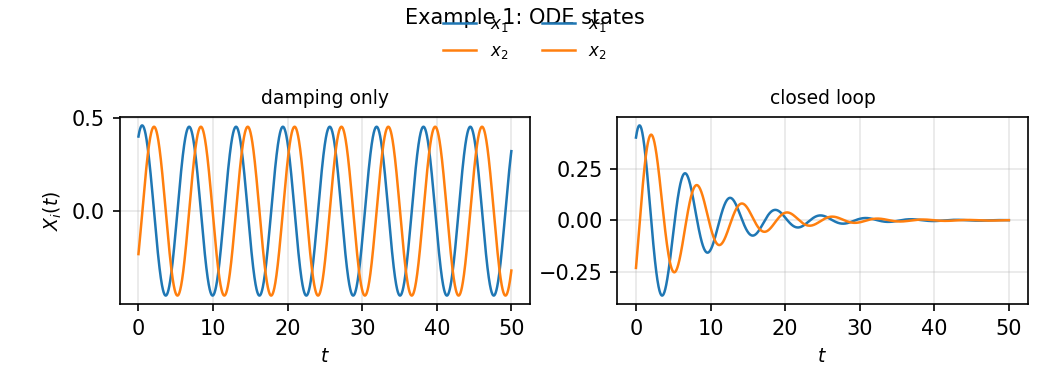
\includegraphics[width=\columnwidth]{fig2.png}}
\caption{Damping-only versus closed-loop ODE state trajectories for Example 1 on
$t \in [0,50]$, using the same initial data in both panels. The left panel
removes the low-gain and stiffness terms and keeps only the boundary damping
term, while the right panel uses the full low-gain feedback law.}
\label{fig2}
\end{figure}

\begin{figure}[!t]
\centerline{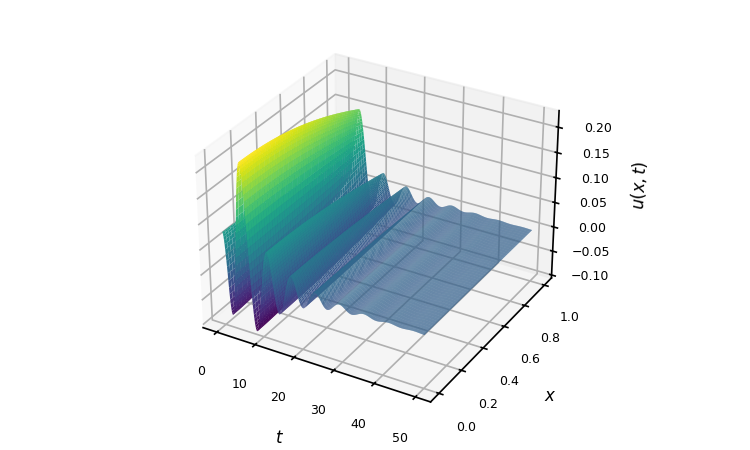
\includegraphics[width=\columnwidth]{fig3.png}}
\caption{Three-dimensional displacement surface for Example 1, showing the
spatiotemporal decay of $u(x,t)$ on $(x,t) \in [0,1]\times[0,50]$.}
\label{fig3}
\end{figure}

Figure~\ref{fig2} directly shows the role of the low-gain component. When only
the boundary damping $U(t) = -u_t(D,t)$ is retained, the two ODE components
remain in a sustained oscillatory regime and do not converge, with
$\Omega(50)/\Omega(0) = 9.27\times 10^{-1}$. Under the full feedback
\eqref{eq:ex1Ctrl}, the closed loop decays. The offline gain is
quadrature-insensitive: computing $B$ on the coarse PDE grid ($N = 200$)
instead of the fine quadrature grid changes \eqref{eq:ex1Bgain} by less than
$10^{-5}$. Quantitatively, the closed-loop energy ratio is
\begin{equation}
\frac{\Omega(50)}{\Omega(0)} = 4.70 \times 10^{-6},
\label{eq:ex1ratio}
\end{equation}
the least-squares semilog decay rate is $0.251$, the $10\%$, $5\%$, and $1\%$
energy thresholds are crossed at $t = 10.4$, $13.3$, and $19.6$, respectively,
and the low-gain component remains moderate with
\begin{equation}
\max_{t\in[0,50]}\abs{B^{\top}P X(t)} = 0.169.
\label{eq:ex1effort}
\end{equation}
Finally, $\abs{X(50)} = 9.22\times 10^{-4}$ and $\abs{u(D,50)} =
1.80\times 10^{-4}$, so the design has entered a clear asymptotic regime within
the window. Figure~\ref{fig3} confirms that the PDE state also decays, in
agreement with Theorem~\ref{thm1}.

\subsection{Example 2: Nilpotent Chain}
\label{ex2}
To illustrate the simplified zero-eigenvalue design, consider the two-
dimensional chain
\begin{equation}
A = \begin{pmatrix} 0 & 1\\ 0 & 0 \end{pmatrix},
\qquad D = 1,\qquad b = 1,\qquad q = 0.5,
\label{eq:ex2A}
\end{equation}
with
\begin{equation}
B_1(x) = \begin{pmatrix} 0\\ 1 \end{pmatrix},
\qquad B_2(x) = 0.
\label{eq:ex2B}
\end{equation}
All eigenvalues of $A$ are at the origin, so this example falls into the
framework of \eqref{eq:nilpBVP}--\eqref{eq:nilpCtrl}. Since $q = 0.5$, the
explicit gain \eqref{eq:nilpB} becomes
\begin{equation}
\bar{B} = \frac{1}{q}\dint{B_1(x)\,\mathrm{d}x} =
\begin{pmatrix} 0\\ 2 \end{pmatrix}.
\label{eq:ex2Bbar}
\end{equation}
Choosing $\varepsilon = 0.20$ gives the Riccati solution of \eqref{eq:are}
\begin{equation}
P_{0.20} = \begin{pmatrix}
0.0020 & 0.0100\\
0.0100 & 0.1000
\end{pmatrix},
\label{eq:ex2P}
\end{equation}
with
\begin{equation}
\bar{B}^{\top}P_{0.20} =
\left(0.0200,\; 0.2000\right),
\label{eq:ex2Pt}
\end{equation}
so the implemented special-case controller is
\begin{equation}
U(t) = -\left(0.0200,\; 0.2000\right)X(t) - u_t(D,t) - 0.5\,u(D,t).
\label{eq:ex2Ctrl}
\end{equation}
The initial conditions $X(0) = (0.30,\,-0.20)^{\top}$, $u(x,0) = 0.04\cos
\frac{\pi x}{2D}$, $u_t(x,0) = 0$ are compatible with the boundary conditions.

\begin{figure}[!t]
\centerline{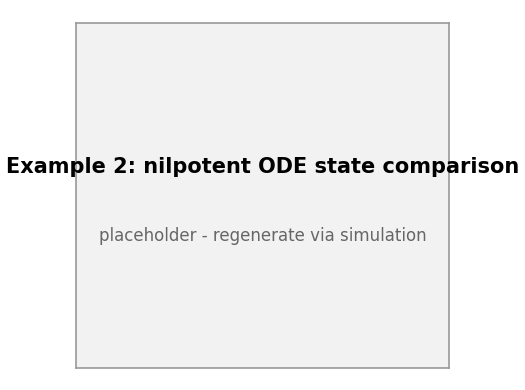
\includegraphics[width=\columnwidth]{fig4.png}}
\caption{Damping-only versus closed-loop ODE state trajectories for the nilpotent
Example 2 on $t \in [0,50]$, using the same initial data in both panels. The left
panel removes the low-gain and stiffness terms and keeps only the boundary
damping term, while the right panel uses the special low-gain feedback law.}
\label{fig4}
\end{figure}

\begin{figure}[!t]
\centerline{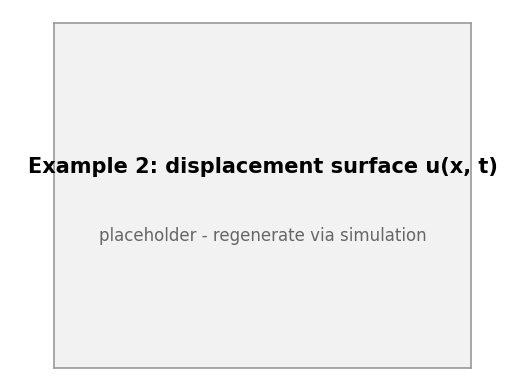
\includegraphics[width=\columnwidth]{fig5.png}}
\caption{Three-dimensional displacement surface for the nilpotent Example 2,
showing the spatiotemporal decay of $u(x,t)$ on $(x,t) \in [0,1]\times[0,50]$.}
\label{fig5}
\end{figure}

Figure~\ref{fig4} shows the same mechanism for the nilpotent chain. Without the
low-gain component the ODE states fail to decay and the chain structure
amplifies the transient. Under the low-gain controller acting through the wave
dynamics, the closed-loop trajectories converge. The observed indicators are
\begin{equation}
\frac{\Omega(50)}{\Omega(0)} = 5.81 \times 10^{-5},
\qquad \max_{t\in[0,50]}\abs{\bar{B}^{\top}P X(t)} = 0.034.
\label{eq:ex2indicators}
\end{equation}
The fitted semilog decay rate is $0.196$, and the energy drops below $10\%$,
$5\%$, and $1\%$ at $t = 9.4$, $9.9$, and $21.3$, respectively. By $t = 50$,
$\abs{X(50)} = 2.68\times 10^{-3}$ and $\abs{u(D,50)} = 6.30\times 10^{-4}$.
Compared with Example~\ref{ex1}, the nilpotent case converges more slowly, which
motivates the longer observation window. Figure~\ref{fig5} shows the
corresponding spatiotemporal decay of the wave state.

Table~\ref{tab1} summarizes the quantitative indicators of both examples.

\begin{table}[!t]
\caption{Simulation indicators for Examples 1 and 2.}
\label{tab1}
\begin{center}
\begin{tabular}{|l|c|c|}
\hline
 & Example 1 & Example 2 \\
\hline
$\varepsilon$ & $0.12$ & $0.20$ \\
$\Omega(50)/\Omega(0)$, closed loop & $4.70\times10^{-6}$ &
$5.81\times10^{-5}$ \\
$\Omega(50)/\Omega(0)$, damping only & $9.27\times10^{-1}$ & $5.40\times10^{2}$ \\
Fitted decay rate & $0.251$ & $0.196$ \\
$10\%/5\%/1\%$ crossing & $10.4/13.3/19.6$ & $9.4/9.9/21.3$ \\
$\max_{t}\abs{KX(t)}$ & $0.169$ & $0.034$ \\
$\abs{X(50)}$ & $9.22\times10^{-4}$ & $2.68\times10^{-3}$ \\
$\abs{u(D,50)}$ & $1.80\times10^{-4}$ & $6.30\times10^{-4}$ \\
\hline
\end{tabular}
\end{center}
\end{table}

\section{Conclusion}
\label{sec:concl}
This paper studied the low-gain stabilization problem for a class of wave
PDE--ODE cascade systems with distributed in-domain displacement and velocity
coupling. By a forwarding-based transformation the distributed input dynamics
reduce to a low-gain design problem with an explicit effective input vector
$B$, and the controller takes the simple form
$U(t) = -B^{\top}P_\varepsilon X(t) - b\,u_t(D,t) - q\,u(D,t)$, combining a
finite-dimensional low-gain term with boundary damping and stiffness; in the
nilpotent case the gain admits the explicit formula \eqref{eq:nilpB}. Under a
low-gain spectral assumption on the ODE dynamics, the closed-loop system is
exponentially stable in a natural energy norm, as proved through a Lyapunov
functional combining the Riccati-based ODE term with the damped wave energy and
suitable cross terms, with the analysis carried out directly on the original
wave state. In comparison with backstepping designs for wave actuator dynamics,
the proposed feedback is much simpler because it uses only the
finite-dimensional state and two local boundary traces online; the price is the
stronger open-loop spectral assumption. Numerical simulations confirm the
theoretical conclusions for both the general and the nilpotent settings. Future
work includes output-feedback designs, robustness with respect to modeling
uncertainty and disturbances, and extensions to more general hyperbolic
actuator dynamics or higher-dimensional distributed systems.

\bibliographystyle{ieeetr}
\bibliography{wave-ode}

\end{document}
